\documentclass{article}
\linespread{1.25}

\usepackage[top = 2cm, right=2cm, left=2cm]{geometry}
\usepackage{graphicx}
\usepackage[section]{placeins}
\usepackage[hidelinks, urlcolor=blue]{hyperref}
\usepackage{float} % for image position in exatly where you want
\usepackage[perpage, stable]{footmisc}
\usepackage{amsmath}
\usepackage{titling}

\usepackage{xepersian}
\settextfont{B Nazanin}
\setlatinmonofont{CMU Serif}
%\setlatinmonofont{Times New Roman}
\setlatintextfont{Times New Roman}

% Set Latin Modern font for the bullets in itemizea
\newfontfamily\latinbullet{Latin Modern Roman}





% Commands
\newcommand{\column}[1]{\lr{\textit{#1}}}
\renewcommand{\labelitemi}{{\latinbullet\textbullet}} % Use the bullet from Latin Modern font

% Custom title page setup
\makeatletter
\def\maketitle{
	\begin{titlepage}
		\begin{center}
			\vspace*{2cm}
			
			{\Large\bfseries درس یادگیری ماشین\par}
			\vspace{2cm}
			
			{\Huge\bfseries گزارش تکلیف
				\lr{Linear Regression}\par}
			\vspace{3cm}
			
			{\large\bfseries استاد درس:\par}
			{\large دکتر افتخاری\par}
			\vspace{1.5cm}
			
			{\large\bfseries نگارش:\par}
			{\large امیرحسین ابوالحسنی\par}
			{\large شماره دانشجویی: 400405003\par}
			\vspace{2cm}
			
			\vfill  % pushes the date to bottom
			
			{\large\bfseries پاییز \lr{1403}}
			
		\end{center}
	\end{titlepage}
	\setcounter{page}{1}
}
\makeatother


\begin{document}
	\maketitle	
	\tableofcontents
	\newpage
	\section{مقدمه
		\footnote{مقدمه با مدل \lr{GPT 3} نوشته شده است.}
	}
	
	رگرسیون خطی یکی از ساده‌ترین و پرکاربردترین روش‌ها در یادگیری نظارت‌شده برای مدل‌سازی رابطه بین یک متغیر وابسته و یک یا چند متغیر مستقل است. با فرض وجود یک رابطه خطی بین ویژگی‌های ورودی و متغیر هدف، رگرسیون خطی تلاش می‌کند بهترین خط را پیدا کند که خطای پیش‌بینی را به حداقل برساند.
	
	هنگامی که تنها یک متغیر مستقل وجود دارد، این روش به عنوان رگرسیون خطی ساده شناخته می‌شود. با این حال، مشکلات دنیای واقعی اغلب شامل چندین عامل مؤثر بر متغیر هدف است. در چنین مواردی از رگرسیون خطی چندگانه استفاده می‌شود، جایی که مدل چندین متغیر مستقل را برای پیش‌بینی متغیر وابسته در نظر می‌گیرد. به صورت ریاضی، این رابطه به صورت زیر مدل‌سازی می‌شود:
	
	\[
	y = w_0 + w_1 x_1 + w_2 x_2 + \dots + w_n x_n + \epsilon
	\]
	
	در اینجا \( y \) مقدار پیش‌بینی‌شده، \( w_0 \) عرض از مبدأ، \( w_1, w_2, \dots, w_n \) ضرایب متغیرهای مستقل \( x_1, x_2, \dots, x_n \)، و \( \epsilon \) خطای مدل است.
	
	در عمل، رگرسیون خطی می‌تواند با استفاده از تکنیک‌های مختلفی حل شود، مانند حل بسته (\lr{closed-form solution}) که از کمینه‌سازی میانگین مربعات خطا (\lr{MSE}) مشتق شده است یا الگوریتم‌های بهینه‌سازی مانند گرادیان نزولی. علاوه بر این، تکنیک‌های تنظیم (\lr{regularization}) مانند تنظیم \( L_2 \) (رگرسیون ریدج) می‌توانند برای جلوگیری از بیش‌برازش با جریمه کردن مقادیر بزرگ ضرایب اعمال شوند. این روش‌ها به‌ویژه در مقابله با چندخطی بودن یا داده‌های پرنویز، پایداری مدل را تضمین می‌کنند.
	
	این گزارش به بررسی رگرسیون خطی ساده و چندگانه می‌پردازد و بر حل بسته در حالت معمولی و با تنظیم $L_2$، بهینه‌سازی گرادیان نزولی در دو حالت گرادیان نزولی تصادفی
	\footnote{\lr{Stochastic Gradient Descent}}
	 و دسته‌ای
	 \footnote{\lr{Batch Gradient Descent}}
	 تاکید دارد.
	  . همچنین عملکرد مدل در روش‌های مختلف با استفاده از داده‌های آموزش و آزمایش مقایسه شده است.
	\section{رگرسیون خطی تک متغیره}
	\subsection{تابع هزینه رگرسیون خطی چیست؟}
	تابع هزینه رگرسیون خطی با نام میانگین مربع خطاها یا 
	\lr{Mean Square Error (MSE)}
	شناخته می‌شود.
	\[J(\theta) = \frac{1}{n}\sum_{i = 1}^n (y^i - \hat{y}^i)^2\]
		
	\subsection{آموزش رگرسیون خطی}
	\subsubsection{راه حل بسته}
	در حل بسته، باید رابطه زیر حل شود تا $\theta$ پیدا شود.
	$$\theta = (X^TX)^{-1}X^T\vec{y}$$
	البته ممکن است
	$X^TX$
	معکوس پذیر نباشد (که در تکلیف همین مورد برای داده‌های \lr{Train} اتفاق می‌افتد.) که در این صورت می توان از \lr{Moore-Penrose pseudo-inverse}
	در رابطه راه حل بسته استفاده کرد:
	$$\theta = (X^TX)^{+}X^T\vec{y}$$
	پاسخ به دست آمده:
	$$
	y = \theta_0 + \theta_1x
	$$
	$$
	\theta_0 = -3.8957 , \theta_1 = 1.1930
	$$
	\newpage
	\subsubsection{گرادیان کاهشی تصادفی}
	در این روش از الگوریتم گرادیان کاهشی تصادفی برای بهینه سازی تابع هزینه استفاده می‌شود.\\
	پاسخ به دست آمده:
	$$
	y = \theta_0 + \theta_1x
	$$
	$$
	\theta_0 = -3.8481, \theta_1 = 1.0570
	$$
	\subsubsection{گرادیان کاهشی دسته‌ای}
	در این روش از الگوریتم گرادیان کاهشی دسته‌ای برای بهینه سازی تابع هزینه استفاده می‌شود.\\
	پاسخ به دست آمده:
	$$
	y = \theta_0 + \theta_1x
	$$
	$$
	\theta_0 = -3.5858, \theta_1 = 1.1619
	$$
	\subsection{مصور سازی مدل با داده‌ها}
	هر سه پاسخ به دست آمده در کنار داده‌ها در شکل 
	\ref{fig: model with data}
	 به تصویر کشیده شده است.‌ همانطور که دیده می شود گرادیان کاهشی دسته‌ای بهتر از تصادفی عمل کرده است.
	\begin{figure}[H]
	 	\centering
	 	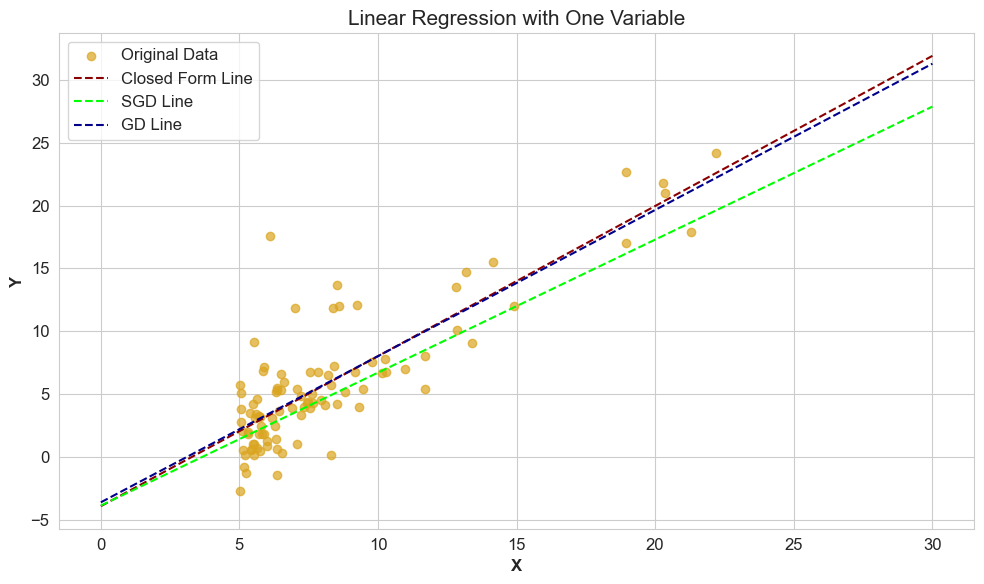
\includegraphics[scale=0.5]{figs/model_with_data}
	 	\caption{خطوط به دست آمده از سه روش مختلف}
	 	\label{fig: model with data}
	\end{figure}
	 
	\subsection{مقایسه پیش‌بینی مدل‌ها}
	پس از آموزش هر مدل، برای تست کردن، به آن‌ها داده‌های 
	\[X = 6.2, 12.8, 22.1, 30\]
	داده می‌شود. نزدیکی خروجی هر مدل، به مدلی که از راه حل بسته به دست آمده است می‌تواند مشخص کند آن شیوه بهینه سازی چقدر خوب توانسته پارامترهایی را پیدا کند که تابع هزینه را کمینه می‌کنند.
	\begin{figure}[H]
		\centering
		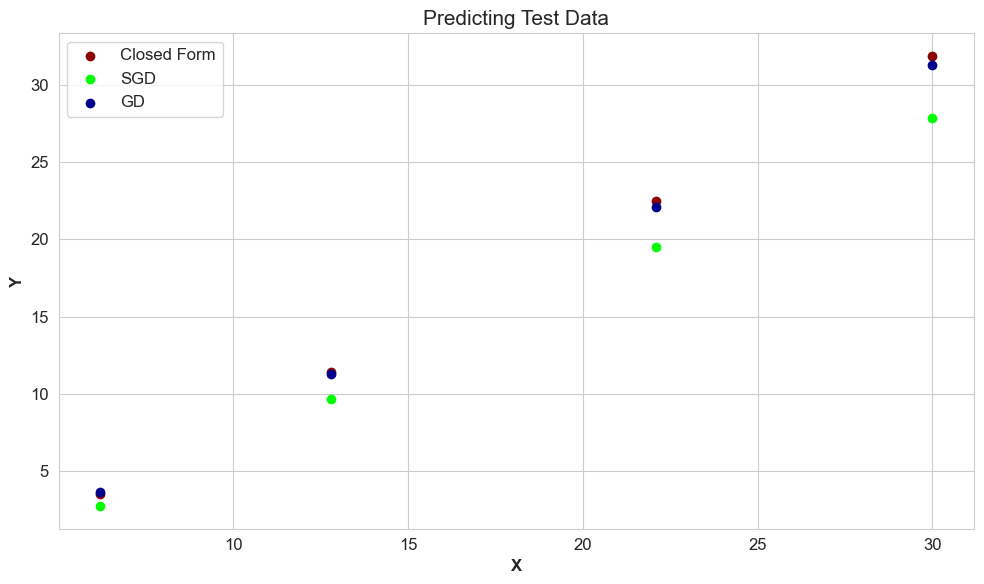
\includegraphics[scale=0.5]{figs/prediction_one_var}
		\caption{خروجی مدل در روش}
		\label{fig: prediction one var}
	\end{figure}
	
		 
	\subsection{مقایسه مدل‌های آموزش دیده}
	از آنحایی که پاسخ بسته بهترین پاسخی است که می‌توان به آن رسید، مقایسه هر خطی با پاسخ بسته می‌تواند نشان بدهد آن مدل چقدر خوب است.(شکل 
	\ref{fig: lines one var}
	)
	\begin{figure}[H]
		\centering
		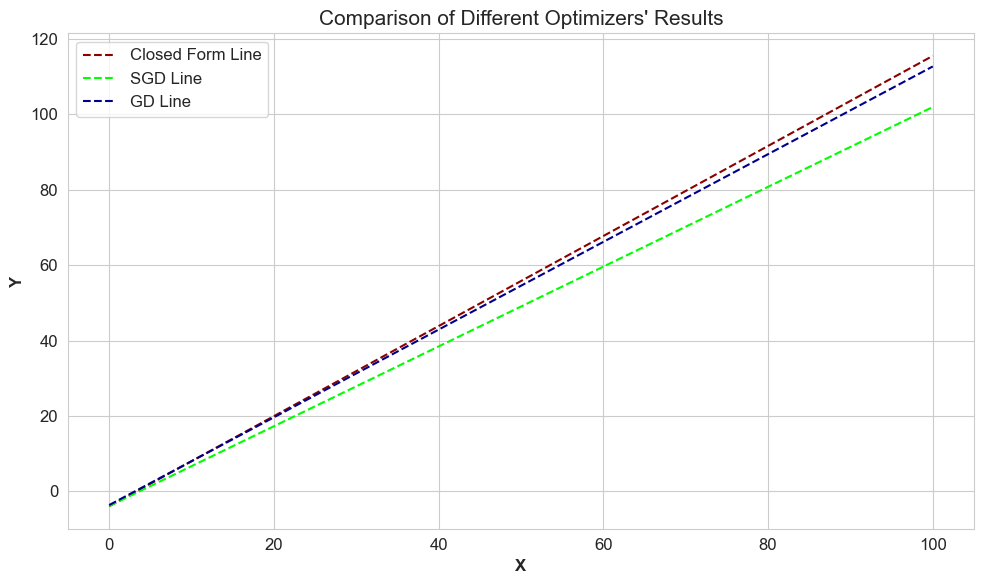
\includegraphics[scale=0.5]{figs/lines_one_var}
		\caption{خروجی مدل در روش}
		\label{fig: lines one var}
	\end{figure}
	
	\subsection{بررسی رفتار تابع هزینه}\label{resuling}
	از مهمترین روش‌های مانیتور کردن کیفیت یادگیری یک مدل، بررسی رفتار تابع هزینه در هنگام آموزش می‌باشد.\\
	همانطور که در شکل
	\ref{fig: cost one var}
	دیده می شود، گرادیان تصادفی بعد از 20 تکرار دیگر نمی‌تواند تابع هزینه را مینیمم کند و احتمالا در یک بهینه محلی گیرکرده است. از طرفی گرادیان کاهشی دسته‌ای توانسته به نزدیکی مقدار مینیمم کلی تابع هزینه برسد.
	\begin{figure}[H]
		\centering
		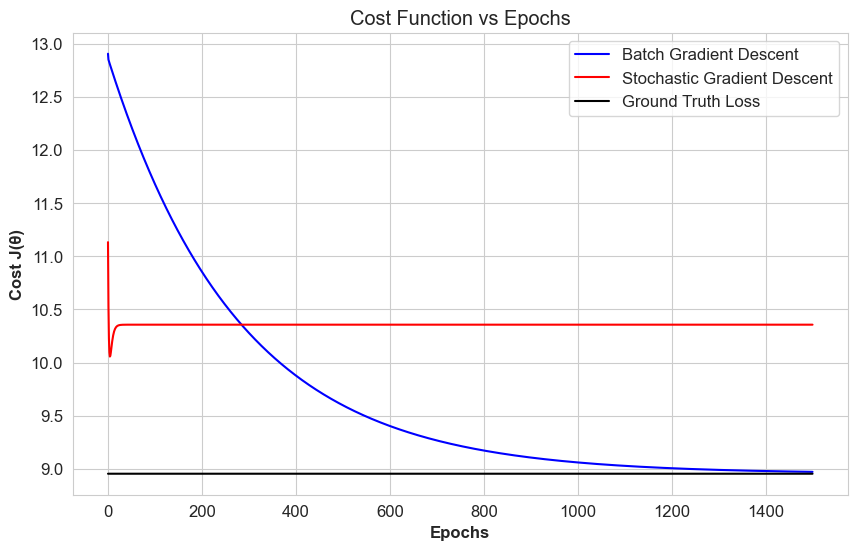
\includegraphics[scale=0.5]{figs/costvsepoch_one_var}
		\caption{نمودار مقدار تابع هزینه با توجه به هر تکرار در زمان یادگیری}
		\label{fig: cost one var}
	\end{figure}
	\subsection{کدام روش بهینه سازی ترجیج داده می‌شود؟}
	با توجه به بخش
	\ref{resuling}	
	و شکل 
	\ref{fig: cost one var}
	می‌توان گفت از آنجایی که گرادیان کاهشی دسته‌ای نسبت به تصادفی بیشتر به کل داده‌ها دید دارد، بهتر می‌تواند مسیر خود را به سمت مینیمم تابع هزینه پیدا کند، مخصوصا زمانی که داده‌ها کم هستند و میتوانند در رم باشند.
	
	\section{رگرسیون چند متغیره}
	\subsection{پیش پردازش‌ داده‌ها}
		\subsubsection{انکود داده‌ها}
		بعضی از متغیر‌های دیتاست کتگوریکال هستند و نیاز بود که اینها متغیر‌ها انکود شوند.
		از \lr{One Hot Encoding (OHE)}
		و 
		\lr{Integer Encoding (IE)}
		برای انکودینگ استفاده شد. متغیر‌
		\column{region}
	با استفاده از \lr{OHE} انکود شده و برای ویژگی‌های 
	\column{smoker, gender}
	از روش دوم انکودیگ استفاده شده است.\\
		\textbf{سوال: چرا برای این سه ویژگی از روش ‌های متفاوت استفاده شد؟}\\
	زمانی از 
	\lr{IE}
	برای انکودیگ استفاده می‌کنیم که بدانیم ترتیب در مقادیر ویژگی مهم است. ممکن است این سوال پیش بیاید که پس چرا برای ویژگی 
	\column{gender}
	از این روش استفاده می‌شود. می‌توان گفت عملا تفاوتی نمی‌کند چون تنها دو مقدار برای این ویژگی وجود دارد.
	و اما زمانی که از روش 
	\lr{OHE}
	استفاده می‌کنیم دیگر ترتیب اثری ندارد و با هر ویژگی ایجاد شده که مقدار 0 یا 1 را دارد به طور عادلانه برخورد می‌شود،‌ همانطور که از ماهیت ویژگی
	\column{region}
	مشخص است.
	
	\subsubsection{استانداردسازی}
	در زمان انجام تکلیف، دیده شد که عدم استانداردسازی داده‌ها باعث انفجار گرادیان و پارامترها می‌شود.
	به همین علت استاندارسازی روی داده‌ها های آموزشی انجام شد و با همان پارامتر‌ها، داده های تست نیز استانداردسازی شدند.
	
	\subsection{پارامتر‌ها با راه حل بسته}
	در این بخش، چون نمی‌توان از $X^TX$ (که $X$ ماتریس داده آموزشی باشد) معکوس گرفت، از
	\lr{Moore-Penrose pseudo-inverse}
	استفاده می‌کنیم.
	
	\subsection{آموزش مدل}
	\subsubsection{گرادیان کاهشی تصادفی}
	\subsubsection{گرادیان کاهشی دسته‌ای}
	\subsubsection{مقایسه روند کاهش تابع هزینه}
	\subsection{اضافه کردن $L_2$ به راه حل بسته}
	
	
	
	
	
		
	
	
	
	
	
	
	
	
	
	
	
	
	
	
	
	
	
	
	
	
	
	
	
	
	
	
	
	
	
	
\end{document}